\documentclass[../DC2017114Bouma.tex]{subfiles}
\graphicspath{{06_Appendices/img/}}
\pagestyle{plain}
\appendix
\renewcommand{\chaptermark}[1]{\markboth{\thechapter.\ #1}{}}
\renewcommand{\sectionmark}[1]{\markright{#1}{}}
\begin{document}

%% New chapter %%
%\pagestyle{fancyreport}
%\cleartooddpage
%\pagestyle{fancyreport}
%\chapter{Mathematical Preliminaries}
%\section{Sensitivity analysis for smooth systems}
%\section{(Non-)linear complementarity problems}
%\section{Convex analysis}
%\section{Hybrid system theory}

%% New chapter %%
\cleartooddpage
\pagestyle{appendix}
\chapter{Nonsmooth modeling}
\section{Discrete event set derivation}\label{app:hybriddisc}
In this section the discrete event sets $D$ are defined. When the state or input of the system enters a discrete event set, contact points can change set and a reinitialization of the state can take place. In this work the assumption is made that all contact points in closed contact are in the same set, i.e., in either $\Ic_{\text{sl}}$ or $\Ic_{\text{st}}$.

\textbf{More elaboration on why the conditions that are chosen are chosen (i.e., why $||\zetab_{t,i}||=0$)}

\textbf{Recap each paragraph using section $D$ and mentioning $\gamma$'s again.}

\textbf{Open to stick/slip}\\
When a contact point is "open", it can trigger a guard function $\gamma_{\text{op}\rightarrow\text{cl}}$ to go from open to closed. This guard is defined using the contact distance $h_{n,i_c}$. When $h_{n,i_c}>0$, the contact point is in open-contact. When $h_{n,i_c}=0$ with $\dot{h}_{n,i_c}<0$, the contact point enters the closed-contact mode with a non-zero ante-impact velocity. Therefore the guard function $\gamma_{\text{op}\rightarrow\text{cl}}$ is given by

\begin{align}
\gamma_{\text{op}\rightarrow\text{cl}} = h_{n,i_c}(\qb).
\end{align}

The plane that spans $\gamma = 0$ is divided in two regions: a region where the post-impact state is in slip and a region where the post-impact state is in stick. $\boldsymbol{I}$ This region is defined by $\Gamma_{i_c}$, where $\Gamma_{i_c}<0$ in the region where the contact point goes to slip and $\Gamma_{i_c} > 0$ in the region where the contact point goes to stick. When $\Gamma_{i_c} = 0$ the system is right at the border between a slip post-impact state and a stick post-impact state. This is illustrated in Figure~\ref{fig:guardopcl}. 
\begin{figure}[H]
	\centering
	\includegraphics[width=.7\textwidth]{guardopcl.eps}\caption{The functions $\gammab(\qb,\dot{\qb})$ and $\Gammab(\qb,\dot{\qb})$ illustrated in the state space of $\qb\in\mathbb{R}^{2}$. The light blue area is the state space where the contact is open, and goes the closed when it triggers $\gamma = 0$. If it triggers $\gamma = 0$ in the area where $\Gamma<0$ (orange), then the contact will go to slip. If it triggers $\gamma=0$ in the area where $\Gamma\geq 0$ (green), then the contact will go to stick.}\label{fig:guardopcl}
\end{figure}
For slip, we know that $\mu\Lambda_{n,i_c} - ||\Lambdab_{t,i_c}|| = 0$ and for stick, we know that  $\mu\Lambda_{n,i_c} - ||\Lambdab_{t,i_c}|| \geq 0$. From this we can derive the guard function
\begin{align}
\Gamma_{i_c} = \mu^2 \underline{\Lambda}_{n,i_c}^2(\underline{\qb},\underline{\dot{\qb}}) - \underline{\Lambdab}_{t,i_c}(\underline{\qb},\underline{\dot{\qb}})\underline{\Lambdab}_{t,i_c}^T(\underline{\qb},\underline{\dot{\qb}}). \label{eq:slipset}
\end{align}
The underlined variables are virtual states, meaning that they do not necessarily have a physical meaning. The way \eqref{eq:slipset} is given, it is defined in both open and closed contact. This map is only physically realistic during an event from open to closed contact. However, by using virtual states we obtain a differentiable guard function $\Gamma_{i_c}$. This guard function $\Gamma_{i_c}$ satisfies the requirements that $\Gamma_{i_c}<0$ in the region where the contact point goes to slip, $\Gamma_{i_c} > 0$ in the region where the contact point goes to stick and $\Gamma_{i_c} = 0$ at the border. We now find expressions for $\Lambda_{n,i_c}$ and $\Lambdab_{t,i_c}$ by looking at the jump map to stick, given in \eqref{eq:appjump5} to \eqref{eq:appjump7}.

We can rewrite \eqref{eq:appjump5} to
\begin{align}
\dot{\qb} = \Mb^{-1}\Wb_{n}\underline{\Lambdab}_{n} + \Mb^{-1}\Wb_{t}\underline{\Lambdab}_{t} + \underline{\dot{\qb}},\label{eq:appqplus}
\end{align}
and \eqref{eq:appjump6}, \eqref{eq:appjump7} to
\begin{align}
\Wb_{n}^T\underline{\dot{\qb}} = 0,\label{eq:appnormalcon}\\
\Wb_{t}^T\underline{\dot{\qb}} = 0,\label{eq:apptangentcon}
\end{align}
with
\begin{align}
\Wb_n &= \begin{bmatrix}
\wb_{n,i_1},\wb_{n,i_2},...,\wb_{n,i_c}
\end{bmatrix}\in\Rbb^{n\times C},\\
\Wb_t &= \begin{bmatrix}
\Wb_{t,i_1},\Wb_{t,i_2},...,\Wb_{t,i_c} 
\end{bmatrix}\in\Rbb^{n\times 2C},\\
\underline{\Lambdab}_n &= \begin{bmatrix}
\underline{\Lambda}_{n,i_1};\underline{\Lambda}_{n,i_2};...;\underline{\Lambda}_{n,i_c} 
\end{bmatrix}\in\Rbb^{C},\\
\underline{\Lambdab}_t &= \begin{bmatrix}
\underline{\Lambdab}_{t,i_1};\underline{\Lambdab}_{t,i_2};...;\underline{\Lambdab}_{t,i_c} 
\end{bmatrix}\in\Rbb^{2C}.
\end{align}
Substituting \eqref{eq:appqplus} into \eqref{eq:appnormalcon} and \eqref{eq:apptangentcon} leads to
\begin{align}
\Wb_{n}^T\Mb^{-1}\Wb_{n}\underline{\Lambdab}_{n} + \Wb_{n}^T\Mb^{-1}\Wb_{t}\underline{\Lambdab}_{t} + \underline{\zetab}_{n} = 0\\
\Wb_{t}^T\Mb^{-1}\Wb_{n}\underline{\Lambda}_{n} + \Wb_{t}^T\Mb^{-1}\Wb_{t}\underline{\Lambdab}_{t} + \underline{\zetab}_{t} = 0,
\end{align}
respectively, with 
\begin{align}
\underline{\zetab}_{n} = \Wb_n^T\underline{\dot{\qb}},\\
\underline{\zetab}_{t} = \Wb_t^T\underline{\dot{\qb}}.
\end{align}
This is now rewritten to
\begin{align}
\begin{bmatrix}
\Wb_{n}^T\Mb^{-1}\Wb_{n} & \Wb_{n}^T\Mb^{-1}\Wb_{t} \\
\Wb_{t}^T\Mb^{-1}\Wb_{n} & \Wb_{t}^T\Mb^{-1}\Wb_{t}
\end{bmatrix}
\begin{bmatrix}
\underline{\Lambdab}_{n}\\
\underline{\Lambdab}_{t}
\end{bmatrix} + \begin{bmatrix}
\underline{\zetab}_{n}\\
\underline{\zetab}_{t}
\end{bmatrix}
= 0,
\end{align}
which is in turn rewritten to
\begin{align}
\begin{bmatrix}
\underline{\Lambdab}_{n}\\
\underline{\Lambdab}_{t}
\end{bmatrix} = - \Db^{-1}\begin{bmatrix}
\underline{\zetab}_{n}\\
\underline{\zetab}_{t}
\end{bmatrix},\quad \text{with } \Db = \begin{bmatrix}
\Wb_{n}^T\Mb^{-1}\Wb_{n} & \Wb_{n}^T\Mb^{-1}\Wb_{t}\\
\Wb_{t}^T\Mb^{-1}\Wb_{n} & \Wb_{t}^T\Mb^{-1}\Wb_{t}
\end{bmatrix}.
\end{align}
The matrix $\Db$ is often called a Delassus-matrix. We now have expressions for $\underline{\Lambdab}_{n}$ and $\underline{\Lambdab}_{t}$ which are continuous and differentiable in $(\qb,\dot{\qb})$. It is straightforward that $\Gamma(\qb,\dot{\qb})$ is continuous and differentiable as well. In this work only trajectories where all closed contacts are in the same mode are considered. This means that when \eqref{eq:slipset} is smaller than zero, i.e., the reaction forces are infeasible for a stick post-impact mode, all contact points have a feasible slip post-impact mode. For trajectories where different contact points can be in slip and in stick at the same time, this conclusion can not be drawn. One should then iterate over all possible post-impact modes until a post-impact mode is found which has feasible reaction forces.

\textbf{Slip to stick/open}\\
When a contact point is in closed-contact slip, it can transition to closed-contact stick and it can transition to open-contact. A slipping contact transitions to sticking when the tangential velocity of the contact point is zero, i.e.,
\begin{align}
||\zetab_{t,\iota}|| = 0.
\end{align}
A guard function that can be used to describe this set is
\begin{align}
\gamma_{\text{sl}\rightarrow\text{st}} = \zetab_{t,\iota}^T\zetab_{t,\iota},
\end{align}
which is equal to zero when $||\zetab_{t,i_c}|| = 0$, greater than zero when $||\zetab_{t,i_c}|| > 0$, smaller than zero when $||\zetab_{t,i_c}|| < 0$, and it is globally differentiable. The time derivative of the guard function is then given by
\begin{align}
\dot{\gamma}^{\text{sl}\rightarrow\text{st}} = \frac{\dot{\zetab}_{t,1} + \dot{\zetab}_{t,2}}{\sqrt{\zetab_{t,1}^2 + \zetab_{t,2}^2}}.
\end{align}
For $\gamma^{\text{sl}\rightarrow\text{st}} = 0$, $\dot{\gamma}^{\text{sl}\rightarrow\text{st}}$ is undefined because of a division by zero. But we can take the left limit of $\dot{\gamma}^{\text{sl}\rightarrow\text{st}}$ to find the direction at which the guard is activated. Using a Taylor expansion w.r.t. the time we can define the limits
\begin{align}
\dot{\zetab}_{t,1}(\tau + s) = a_1 s + o(s),\\
\dot{\zetab}_{t,2}(\tau + s) = a_2 s + o(s),
\end{align}
where $\tau$ is the event time where $\gamma = 0$. Note that the Taylor expansions are only physically realistic for $s < 0$. We can then write
\begin{align}
\dot{\gamma}^{\text{sl}\rightarrow\text{st}}(\tau+s) = \frac{(a_1 + a_2)s + o(s)}{\sqrt{(a_1^2 + a_2^2)s^2 + o(s^2)}} \approx \Sign(s)(a_1 + a_2).
\end{align}
Since we're interested in the left limit, we get
\begin{align}
\lim\limits_{s\rightarrow 0^-}\dot{\gamma}^{\text{sl}\rightarrow\text{st}}(\tau+s) = -(a^2_1 + a^2_2),
\end{align}
which will be non-zero when the guard is activated transversally. This guard function can be used to perform the positive homogenization. For simulations we have to find another solution, because $\gamma^{\text{sl}\rightarrow\text{st}}$ cannot become negative. This will lead to problems when we use zero-border crossing detection.

For a slipping contact transitioning to open-contact an acceleration based guard function is necessary, since the normal velocity of the contact point is constrained in the continuous dynamics of a slipping contact. Therefore, a slipping contact point transitions to open-contact when
\begin{align}
\lambda_{n,i_c} = 0.\label{eq:applambdanguard}
\end{align}
Similarly to the expression found for $\Lambdab_{n}$ and $\Lambdab_{t}$, we can use \eqref{eq:qddot} and \eqref{eq:fcontconst} to define the vector $\lambdab_{n}$. With
\begin{align}
\underline{\lambdab}_n &= \begin{bmatrix}
\underline{\lambda}_{n,i_1};\underline{\lambda}_{n,i_2};...;\underline{\lambda}_{n,i_C} 
\end{bmatrix}\in\Rbb^{C},\\
\underline{\lambdab}_t &= \begin{bmatrix}
\underline{\lambdab}_{t,i_1};\underline{\lambdab}_{t,i_2};...;\underline{\lambdab}_{t,i_C} 
\end{bmatrix}\in\Rbb^{2C},
\end{align}
the dynamics and constraints for a system with all closed contact points in slip are defined as
\begin{align}
&\ddot{\qb} = \Mb^{-1}\left[\Sb\ub - \Hb + \Wb_{n}\lambdab_{n} + \Wb_{t}\lambdab_{t}\right],\label{eq:appslipdyn1}\\
&\Wb^T_{n}\ddot{\qb} + \dot{\Wb}^T_{n}\dot{\qb} = 0,\label{eq:appslipdyn2}\\
&\lambdab_{t} = -\mu\Zb_{t}\lambdab_{n},\label{eq:appslipdyn3}
\end{align}
with 
\begin{align}
\Zb_{t} = \begin{bmatrix}
\langle\zetab_{t,i_1}\rangle & \mathbf{0} & \cdots & \mathbf{0}\\
\mathbf{0} & \langle\zetab_{t,i_2}\rangle & \cdots & \mathbf{0}\\
\vdots & \vdots & \ddots & \vdots\\
\mathbf{0} & \mathbf{0} & \cdots & \langle\zetab_{t,i_C}\rangle
\end{bmatrix},\quad\in\Rbb^{2C \times C}\label{eq:appZt}
\end{align}
where $\langle\zetab_{t}\rangle=\begin{bmatrix}\langle\zetab_{t,i_1}\rangle,\langle\zetab_{t,i_2}\rangle,...,\langle\zetab_{t,i_C}\rangle \end{bmatrix}^T$, with $\langle\zetab_{t,i_c}\rangle$ the unit vector $\zetab_{t,i_c}$. \eqref{eq:appslipdyn1}-\eqref{eq:appslipdyn3} can be rewritten into
\begin{align}
&\lambdab_{n} = -\left[\Wb^T_{n}\Mb^{-1}\left(\Wb_{n} - \mu\Wb_{t}\Zb_{t}\right)\right]^{-1}\Wb^T_{n}\Mb^{-1}\left[\Sb\ub - \Hb\right] - \dot{\Wb}^T_{n}\dot{\qb},
\end{align}
which can be used to define the guard function \eqref{eq:applambdanguard}.

\textbf{Stick to slip/open}\\
When a contact point is in closed-contact stick, it can transition to closed-contact slip and it can transition to open-contact. A slipping contact transitions to sticking when the tangential reaction force becomes equal to the normal reaction force at that contact point times the friction coefficient, i.e.,
\begin{align}
\mu\lambda_{n,i_c} = ||\lambdab_{t,i_c}||.
\end{align}
A guard function that can be used to describe this set is
\begin{align}
\gamma_{\text{st}\rightarrow\text{sl}} = \mu^2\lambda^2_{n,i_c} - \lambdab_{t,i_c}\lambdab_{t,i_c}^T,\label{eq:appguardstsl}
\end{align}
which is equal to zero when $\mu^2\lambda^2_{n,i_c} = ||\lambdab_{t,i_c}||$, greater than zero when $\mu^2\lambda^2_{n,i_c} > ||\lambdab_{t,i_c}||$, and it is globally differentiable. It is physically impossible that $\mu^2\lambda^2_{n,i_c} < ||\lambdab_{t,i_c}||$, meaning that $\gamma_{\text{st}\rightarrow\text{sl}}$ will never be smaller than zero. The dynamics and constraints of a system with all contact points in stick are defined as
\begin{align}
&\ddot{\qb} = \Mb^{-1}\left[\Sb\ub - \Hb + \Wb_{n}\lambdab_{n} + \Wb_{t}\lambdab_{t}\right],\label{eq:appstickdyn1}\\
&\Wb^T_{n}\ddot{\qb} + \dot{\Wb}^T_{n}\dot{\qb} = 0,\label{eq:appstickdyn2}\\
&\Wb^T_{t}\ddot{\qb} + \dot{\Wb}^T_{t}\dot{\qb} = 0,,\label{eq:appstickdyn3}
\end{align}
Substituting \eqref{eq:appstickdyn1} into \eqref{eq:appstickdyn2} and \eqref{eq:appstickdyn3} leads to
\begin{align}
\Wb_{n}^T\Mb^{-1}\Wb_{n}\lambdab_{n} + \Wb_{n}^T\Mb^{-1}\Wb_{t}\lambdab_{t} = \Wb_{n}^T\Mb^{-1}\left[\Sb\ub - \Hb\right] -\dot{\Wb}^T_{n}\dot{\qb}, \\
\Wb_{t}^T\Mb^{-1}\Wb_{n}\lambdab_{n} + \Wb_{t}^T\Mb^{-1}\Wb_{t}\lambdab_{t} = \Wb_{t}^T\Mb^{-1}\left[\Sb\ub - \Hb\right] -\dot{\Wb}^T_{t}\dot{\qb},
\end{align}
which can be rewritten to
\begin{align}
\begin{bmatrix}
\lambdab_{n}\\
\lambdab_{t}
\end{bmatrix} = - \Db^{-1}\begin{bmatrix}
\Wb_{n}^T\Mb^{-1}\left[\Sb\ub - \Hb\right] -\dot{\Wb}^T_{n}\dot{\qb}\\
\Wb_{t}^T\Mb^{-1}\left[\Sb\ub - \Hb\right] -\dot{\Wb}^T_{t}\dot{\qb}
\end{bmatrix}.\label{eq:applambdastick}
\end{align}

Using \eqref{eq:applambdastick} the guard function \eqref{eq:appguardstsl} is defined.

\section{Proximal Point Formulation}
The contact law and friction law defined in the complementarity condition formulation can be redefined to a proximal point formulation. This makes the system compatible with simulation methods as timestepping \cite[Chapter 10]{Acary2008}. More information on the definition of the proximal point formulation of contact laws and friction laws can be found in \cite[Section 5.3]{Leine2008}.

\subsection{Signorini's contact law and Poisson's impact law}
In Figure~\ref{fig:convex} a convex set $C$ is illustrated. The normal cone $N_C(\xb)$ of a point $\xb$ is $N_C(\xb)=0$ if $\xb\in \text{int}(C)$, where $\text{int}(.)$ is the interior of a set. An example of this is point $\xb_3$ in Figure~\ref{fig:convex}. Defining $\text{bd}(.)$ as the boundary of the set, when $\xb\in \text{bd}(C)$ there are two options. When $\xb$ is on a smooth part of $\text{bd}(C)$, then $N_C(\xb)$ is a ray normal to $\text{bd}(C)$ at point $\xb$ as depicted in at point $\xb_1$. When $\xb$ is on a nonsmooth part of $\text{bd}(C)$, then $N_C(\xb)$ is a cone starting on the point $\xb$ whose sides are normal to the left and right approximation of the point $\xb$ on $\text{bd}(C)$. This is illustrated at point $\xb_2$. The proximal point $\prox_C(\zb)$ of a point $\zb$, is the point in $C$ closest to the point $\zb$. The point $\xb$ is the proximal point to all points  $\zb\in N_C(\xb)$. For a point $\zb\in C$, $\prox_C(\zb) = \zb$ i.e. $\xb_3$ in Figure~\ref{fig:convex}.

\begin{figure}[h]
\centering
\includegraphics[width=.6\textwidth]{convex.PNG}\caption{}\label{fig:convex}
\end{figure}

This formulation can be used to define Signorini's contact law, which is defined as \eqref{eq:ncpcontact2}. The normal cone formulation, as illustrated in Figure~\ref{fig:convex}, of the contact is given by

\begin{align}
-h_{n,i} \in N_{C_{n,i}}(\lambda_{n,i}),\quad \text{with }C_{n,i} = (\Rbb^n)^+.\label{eq:hnormalcone}
\end{align}
The set $C_{n,i}$ is the set of admissible normal forces according to Signorini's law. See Figure~\ref{fig:signorinicontact} for an illustration of the set $C_{n,i}$ with $\lambda_{n,i}\in C_{n,i}$ and $h_{n,i} \in N_{C_{n,i}}(\lambda_{n,i})$. Now using the fact that
\begin{align}
\xb = \prox_C(\xb -r\yb), r > 0\ \iff\ -\yb\in N_C(\xb),
\end{align}
rewriting \eqref{eq:hnormalcone} to a proximal point formulation gives 

\begin{align}
\lambda_{n,i} = \prox_{C_{n,i}}(\lambda_{n,i} - rh_{n,i}),\quad \text{with }C_{n,i} = (\Rbb^n)^+\text{ and } r>0.
\end{align}

Similarly for the Poisson's impact law illustrated in Figure~\ref{fig:poissonimpact}, we find the proximal point formulation

\begin{align}
\Lambda_{n,i} = \prox_{C_{n,i}}(\Lambda_{n,i} - r\zeta^+_{n,i}),\quad \text{with }C_{n,i} = (\Rbb^n)^+\text{ and } r>0.
\end{align}

\subsection{Coulomb's friction law}
Now we define the normal cone formulation of Coulomb's friction law
\begin{align}
-\zetab_{t,i} \in N_{C_{t,i}}(\lambdab_{t,i})\quad \forall i\in\Ic_a,\quad \text{with }C_{t,i}(\lambda_{n,i}) = \{\lambdab_{t,i}\ |\ ||\lambdab_{t,i}|| \leq \mu\lambda_{n,i}\},
\end{align}
which is illustrated in Figure~\ref{fig:frictiondisk}.  

\begin{figure}[h]
\centering
\includegraphics[width=.4\textwidth]{frictiondisk.eps}\caption{The friction disk with two seperate friction forces $\lambdab_{t,1}$ and $\lambdab_{t,2}$. $\lambdab_{t,1} = \mu\lambda_{n,1}$, resulting in a tangential velocity $\zetab_{t,i}>0$. $\lambdab_{t,2}<\mu\lambda_{n,2}$, leading to a tangential velocity $\zetab_{t,i}=0$.}\label{fig:frictiondisk}
\end{figure}

$C_t$ is the set of all admitted friction forces. The tangential velocity $\zetab_{t,i}$ is directed opposite to the friction force $\lambdab_{t,i}$ for isotropic friction. 

Now using the fact that
\begin{align}
\xb = \prox_C(\xb -r\yb), r > 0\ \iff\ -\yb\in N_C(\xb),
\end{align}
we can rewrite the normal cone to a proximal point formulation
\begin{align}
\lambdab_{t,i} = \prox_{C_{t,i}}(\lambdab_{t,i} - r\zetab_{t,i})\,\quad\text{with }C_{t,i}(\lambda_{n,i}) = \{\lambdab_{t,i}\ |\ ||\lambdab_{t,i}|| \leq \mu\lambda_{n,i}\}\text{ and }r>0.
\end{align}
Similarly, for the impact dynamics we can formulate
\begin{align}
\Lambdab_{t,i} = \prox_{C_{t,i}}(\Lambdab_{t,i} - r\zetab^+_{t,i})\,\quad \text{with }C_{t,i}(\lambda_{n,i}) = \{\Lambdab_{t,i}\ |\ ||\Lambdab_{t,i}|| \leq \mu\Lambda_{n,i}\}\text{ and }r>0.
\end{align}

\subsection{System dynamics with contact law and friction law}
The flow dynamics is then described by
\begin{align}
&\Mb(\qb)\dot{\xib} + \Hb(\qb,\xib) = \Sb(\qb)\ub + \sum_{i\in\Ic_c}\left(\wb_{n,i}(\qb)\lambda_{n,i} + \Wb_{t,i}(\qb)\lambdab_{t,i} \right), \label{eq:proxcontact1}\\
&\lambda_{n,i} = \prox_{C_{n,i}}(\lambda_{n,i} - rh_{n,i}),\label{eq:proxcontact2}\\
&\lambdab_{t,i} = \prox_{C_{t,i}}(\lambdab_{t,i} - r\zetab_{t,i}),\label{eq:proxcontact3}
\end{align}
with
\begin{align}
&C_{n,i} = (\Rbb^n)^+\text{ and } r>0,\\
&C_{t,i}(\lambda_{n,i}) = \{\lambdab_{t,i}\ |\ ||\lambdab_{t,i}|| \leq \mu\lambda_{n,i}\}\text{ and }r>0.
\end{align}
The impulsive dynamics that take place when a contact point opens or closes contact is described by
\begin{align}
&\Mb(\qb)(\xib^+ - \xib^-) = \sum_{i\in\Ic_c}\left( \wb_{n,i}(\qb)\Lambda_{n,i} + \Wb_{t,i}(\qb)\Lambdab_{t,i}\right), \label{eq:proximpact1}\\
&\Lambda_{n,i} = \prox_{C_{n,i}}(\Lambda_{n,i} - r\zeta^+_{n,i}),\label{eq:proximpact2}\\
&\Lambdab_{t,i} = \prox_{C_{t,i}}(\Lambdab_{t,i} - r\zetab^+_{t,i})\,\label{eq:proximpact3}
\end{align}
with
\begin{align}
&C_{n,i} = (\Rbb^n)^+\text{ and } r>0,\\
&C_{t,i}(\lambda_{n,i}) = \{\Lambdab_{t,i}\ |\ ||\Lambdab_{t,i}|| \leq \mu\Lambda_{n,i}\}\text{ and }r>0.
\end{align}

%% New chapter %%
\pagestyle{fancyreport}
\cleartooddpage
\pagestyle{fancyreport}
\chapter{Frictional Impacts in Mechanical Systems}
\section{Reference trajectories with impact away from slip-stick border}\label{app:impactsaway}
Now we look at the case where a contact point goes from open to closed, away from $\Gammab = 0$. This is illustrated in Figure~\ref{fig:impactfromborder}. The goal is to prove that for an event away from $\Gammab$, a sufficiently small perturbation cannot cause the trajectory to hit $\gamma = 0$ at a perturbed ante-impact state $\xb_\epsilon^-(t_\epsilon)$ where $\Gammab$ changes sign in comparison with the unperturbed ante-impact state $\alphab^-(\tau)$. From \cite[p. 6]{Rijnen2018} we know that based on the continuity property of $\gammab$ and $\fb$, the perturbed impact state can be written as

\begin{align}
\xb_\epsilon(t_\epsilon) = \alphab(\tau) + \epsilon\dot{\alphab}(\tau)\frac{\partial t_\epsilon}{\partial \epsilon} + \epsilon\zb(\tau) + o(\epsilon),\label{eq:appxpert}
\end{align}
for sufficiently small $\epsilon$. The shortest distance between $\Gammab = \Gammab(\alphab(\tau))$ and $\Gammab = 0$ on the plane where $\gammab = 0$ is defined as the constant $\delta_{\Gammab}$, which is also illustrated in Figure~\ref{fig:impactfromborder}.

\begin{figure}[h]
\centering
\includegraphics[width=.5\textwidth,trim={0cm 2.5cm 2cm 2.4cm},clip]{impactfromborder.eps}\caption{The guard functions $\gammab$ and $\Gammab$ in the state space of $\qb$. A transition from open to closed is made away from $\Gammab$. $\alphab(t)$ is the nominal trajectory and $\xb_\epsilon(t)$ a perturbed trajectory of the contact point up to the transition.} \label{fig:impactfromborder}
\end{figure}

Let's define a point in the state $\xb_{\gammab=0,\Gammab=0}$ where $\gammab(\xb_{\gammab=0,\Gammab=0})=0$ and $\Gammab(\xb_{\gammab=0,\Gammab=0})=0$. We are evaluating nominal trajectories which impact away from $\Gammab = 0$, i.e. $\Gammab(\alphab(\tau))\neq \Gammab(\xb_{\gammab=0,\Gammab=0})$. From Section~\ref{app:guards} we know that $\Gammab$ is continuously differentiable, which implies that it is Lipschitz-continuous and therefore satisfies the Lipschitz-continuity condition

\begin{align}
||\fb(\xb)-\fb(\yb)|| \leq \kappa||\xb-\yb||,\quad \forall \xb,\yb\in\Rbb^n,\label{eq:appLipschitz}
\end{align}
where $\kappa>0$ \cite{Leine2008}. By applying \eqref{eq:appLipschitz} to the function value of $\Gammab$ at impact for the nominal trajectory and the perturbed trajectory, we find

\begin{align}
||\Gammab(\alphab(\tau)) - \Gammab(\xb_{\gammab=0,\Gammab=0})||\leq \kappa||\alphab(\tau)-\xb_{\gammab=0,\Gammab=0}||.\label{eq:appLipschitz2}
\end{align}
Now, since $\Gammab(\alphab(\tau))\neq \Gammab(\xb_{\gammab=0,\Gammab=0})$, we know that $||\Gammab(\alphab(\tau)) - \Gammab(\xb_{\gammab=0,\Gammab=0})||>0$ and therefore from \eqref{eq:appLipschitz2} that $||\alphab(\tau)-\xb_{\gammab=0,\Gammab=0}||>0$, i.e. $\delta_{\Gammab} >0$. Finally, from \eqref{eq:appxpert}, we find

\begin{align}
||\xb_\epsilon(t_\epsilon) - \alphab(\tau)|| = ||\epsilon\dot{\alphab}(\tau)\frac{\partial t_\epsilon}{\partial \epsilon} + \epsilon\zb(\tau) + o(\epsilon)||.
\end{align}
Since $\delta_{\Gammab} > 0$ and $\lim_{\epsilon\rightarrow 0}||\xb_\epsilon(t_\epsilon) - \alphab(\tau)||=0$, there always exists an $\epsilon$ such that $||\xb_\epsilon(t_\epsilon) - \alphab(\tau)||<\delta_{\Gammab}$. 

In other words, this proves that if $\fb$, $\gammab$ and $\Gammab$ are continuous and the nominal trajectory makes impact away from the slip-stick post-impact mode border $\Gammab = 0$, then there always exists a range of $\epsilon$ such that the perturbed state will have the same post-impact mode as the nominal trajectory.

\section{Post-impact accelerations in open-to-stick transitions}
The mode transition from stick to slip happens when a guard is triggered at acceleration level, 
\begin{align}
^{\text{slip}\leftarrow\text{stick}}\gamma = \mu^2\lambda_{n,i}^2 - \lambdab_{t,i}\lambdab_{t,i}^T,
\end{align}
and the post-impact mode is determined by the guard function defined at velocity level
\begin{align}
\Gamma = \mu^2 \Lambda_{n,i}^2(\qb,\dot{\qb}^-) - \Lambdab_{t,i}(\qb,\dot{\qb}^-)\Lambdab_{t,i}^T(\qb,\dot{\qb}^-). \label{eq:appopentostick}
\end{align}
Since the jump map from open to stick is
\begin{align}
&\Mb(\qb)(\dot{\qb}^+ - \dot{\qb}^-) = \wb_{n,i}(\qb)\Lambda_{n,i} + \Wb_{t,i}(\qb)\Lambdab_{t,i},\label{eq:appjump8}\\
&\zeta_{n,i}^+ = 0,\label{eq:appjump9}\\
&\zeta_{t,i}^+ = 0,\label{eq:appjump10}
\end{align}
which is on velocity level, the post-impact reaction forces of the open-to-stick event can be in the stick-to-slip jump set, causing an immediate transition to slip. This is demonstrated using the flow dynamics of the stick mode at the time-instant of the transition,
\begin{align}
&\Mb(\qb^+)\ddot{\qb}^+ + \Hb(\qb^+,\dot{\qb}^+) = \Sb(\qb^+)\ub^+ + \sum_{i\in\Ic_c}\left(\wb_{n,i}(\qb^+)\lambda^+_{n,i} + \Wb_{t,i}(\qb^+)\lambdab^+_{t,i} \right), \label{eq:appstickdyn+1}\\
&\wb^T_{n,i}(\qb^+)\ddot{\qb}^+ + \dot{\wb}^T_{n,i}(\qb^+)\dot{\qb}^+ = 0,\label{eq:appstickdyn+2}\\
&\Wb^T_{t,i}(\qb^+)\ddot{\qb}^+ + \dot{\Wb}^T_{t,i}(\qb^+)\dot{\qb}^+ = 0.\label{eq:appstickdyn+3}
\end{align}

We can deduce from \eqref{eq:appjump9}-\eqref{eq:appjump10} and \eqref{eq:appstickdyn+2}-\eqref{eq:appstickdyn+3} that the normal acceleration of the transition contact point $\wb^T_{n,i}(\qb^+)\ddot{\qb}^+$ and the tangential acceleration of the transitioning contact point $\Wb^T_{t,i}(\qb^+)\ddot{\qb}^+$ are both equal to zero. From \eqref{eq:appstickdyn+1} we then notice that $\lambda_{n,i}^+$ and $\lambdab_{t,i}^+$ depend continuously on $\ub^+$ and can therefore instantly lead to $\mu^2\lambda_{n,i}^2 - \lambdab_{t,i}\lambdab_{t,i}^T>0$ for certain $\ub^+$. For these inputs the contact point will immediately start slipping after the open-to-stick transition. These areas are illustrated in Figure~\ref{fig:stickimmedslip}

\begin{figure}[h]
\centering
\includegraphics[width=.55\textwidth]{stickimmedslip.eps}\caption{The border between an open-to-stick event that stays in stick and an open-to-stick event that immediately starts slipping is illustrated in this figure. The post event state and input indicated in the figure is in the $\mu^2(\lambda^+_{n,i})^2 - \lambdab^+_{t,i}(\lambdab^+_{t,i})^T > 0$ area, causing the contact point to immediately start slipping.} \label{fig:stickimmedslip}
\end{figure}

Using the continuity of the system's flow dynamics and the function $\mu^2(\lambda^+_{n,i})^2 - \lambdab^+_{t,i}(\lambdab^+_{t,i})^T$, we can show that if we choose $\mub^+$ such that $\alphab^+,\mub^+$ is not on $\mu^2(\lambda^+_{n,i})^2 - \lambdab^+_{t,i}(\lambdab^+_{t,i})^T = 0$ then there always exists a range of perturbations $\epsilon$ such that the perturbed post-impact is on the same side of $\mu^2(\lambda^+_{n,i})^2 - \lambdab^+_{t,i}(\lambdab^+_{t,i})^T = 0$ as the unperturbed trajectory similarly to Section~\ref{app:impactsaway}.

%% New chapter %%
\pagestyle{fancyreport}
\cleartooddpage
\pagestyle{fancyreport}
\chapter{Sensitivity Analysis for Input-Dependent Guards}\label{app:Csensitivity}
\section{Linearized jump gain for isolated events}
The perturbed state is defined as
\begin{align}
\xb(t,\epsilon) = \xb(t_0,\epsilon) + \int_{t_0}^{t}\fb(\xb(s,\epsilon),\ub(s,\epsilon),s)ds.
\end{align}
Then
\begin{align}
\frac{\partial\xb(t,\epsilon)}{\partial\epsilon} &= \frac{\partial\xb_0}{\partial\epsilon} + \int_{t_0}^{t}\left(\frac{\partial\fb}{\partial\xb}\frac{\partial\xb}{\partial\epsilon} + \frac{\partial\fb}{\partial\ub}\frac{\partial\ub}{\partial\epsilon}\right)ds,\\
\frac{\partial^2\xb}{\partial t\partial\epsilon} &= \frac{\partial\fb}{\partial\xb}\frac{\partial\xb}{\partial\epsilon} + \frac{\partial\fb}{\partial\ub}\frac{\partial\ub}{\partial\epsilon},
\end{align}
which we can write as
\begin{align}
\frac{\partial^2\xb}{\partial t\partial\epsilon} = D_1\fb(\xb(t,\epsilon),\ub(t,\epsilon),t)\cdot \frac{\partial\xb}{\partial\epsilon} + D_2\fb(\xb(t,\epsilon),\ub(t,\epsilon),t)\cdot \frac{\partial\ub}{\partial\epsilon}, \label{eq:dxdtde}
\end{align}
with $D_i\fb$ the derivative of $\fb$ wrt the $i$th term of $\fb$. Evaluating \eqref{eq:dxdtde} at $\epsilon = 0$ results in the flow dynamics of the positive homogenization
\begin{align}
\dot{\zb} = D_1\fb(\alphab(t),\mub(t),t)\cdot \zb(t) + D_2\fb(\alphab(t),\mub(t),t)\cdot \vb(t),
\end{align}
where 
\begin{align}
\zb(t) = \left.\frac{\partial\xb(t,\epsilon)}{\partial\epsilon}\right|_{\epsilon=0},\text{ and } \vb(t) = \left.\frac{\partial\ub(t,\epsilon)}{\partial\epsilon}\right|_{\epsilon=0} .
\end{align}
When we consider a single jump
\begin{align}
\xb^{+}_\epsilon(t_\epsilon,\epsilon) = \gb(\xb^{-}_\epsilon(t_\epsilon,\epsilon),t_\epsilon),\label{eq:g}
\end{align}
using a Taylor approximation on the left-hand side of \eqref{eq:g} with respect to $\epsilon$ and around $\epsilon = 0$, we can write
\begin{align}
\xb^{+}_\epsilon(t_\epsilon,\epsilon) &= \alphab^{+}(t_\epsilon) + \epsilon \zb^{+}(t_\epsilon) + o(\epsilon),\label{eq:xe}\\
\ub^{+}_\epsilon(t_\epsilon,\epsilon) &= \mub^{+}(t_\epsilon) + \epsilon \vb^{+}(t_\epsilon) + o(\epsilon),\label{eq:ue}
\end{align}
where $\alphab(t)$ is a nominal reference trajectory that satisfies the dynamics of the system and $\mub(t)$ an input that achieves this reference trajectory. Now we expand this in terms of $\epsilon$, so with
\begin{align}
\Delta = \left.\frac{\partial t_\epsilon}{\partial\epsilon}\right|_{\epsilon=0},
\end{align} 
we get
\begin{align}
\alphab^{+}(t_\epsilon) &= \alphab^{+}(\tau) + \epsilon \dot{\alphab}^{+}(\tau)\Delta + o(\epsilon),\\
\mub^{+}(t_\epsilon) &= \mub^{+}(\tau) + \epsilon \dot{\mub}^{+}(\tau)\Delta + o(\epsilon),\\
\zb^{+}(t_\epsilon) &= \zb^{+}(\tau) + \epsilon \dot{\zb}^{+}(\tau)\Delta + o(\epsilon),\\
\vb^{+}(t_\epsilon) &= \vb^{+}(\tau) + \epsilon \dot{\vb}^{+}(\tau)\Delta + o(\epsilon),
\end{align}
which when substituted into \eqref{eq:xe} and \eqref{eq:ue} gives,
\begin{align}
\xb^{+}_\epsilon(t_\epsilon,\epsilon) &= \alphab^{+}(\tau) + \epsilon \dot{\alphab}^{+}(\tau)\Delta + \epsilon \zb^{+}(\tau) + o(\epsilon). \label{eq:xeexp}\\
\ub^{+}_\epsilon(t_\epsilon,\epsilon) &= \mub^{+}(\tau) + \epsilon \dot{\mub}^{+}(\tau)\Delta + \epsilon \vb^{+}(\tau) + o(\epsilon). \label{eq:ueexp}
\end{align}
 To find $\Delta$, we evaluate the ante impact guard function
\begin{align}
\gamma^{-}( \xb^{-}_\epsilon(t_\epsilon),\ub^{-}_\epsilon(t_\epsilon),t_\epsilon) = 0.
\end{align}
In previous work, the guard function $\gamma$ was not dependent on $\ub_\epsilon(t_\epsilon)$ because friction and release was not considered. We now expand $\gamma(\xb_\epsilon(t_\epsilon),\ub_\epsilon(t_\epsilon),t_\epsilon)$ wrt $\epsilon$, giving
\begin{align}
\gamma&(\xb_\epsilon(t_\epsilon),\ub_\epsilon(t_\epsilon),t_\epsilon) = \gamma( \alphab(\tau), \mub(\tau),\tau) + \epsilon\left[\frac{\partial \gamma}{\partial\epsilon}(\alphab(\tau),\mub(\tau),\tau)\right]_{\epsilon=0} + o(\epsilon),\\
&= \gamma( \alphab(\tau), \mub(\tau),\tau) + \epsilon\left[ \frac{\partial\gamma}{\partial\xb}\left(\frac{\partial\xb}{\partial\epsilon} + \frac{\partial\xb}{\partial t_\epsilon}\frac{d t_\epsilon}{d\epsilon}\right) + \frac{\partial\gamma}{\partial\ub}\left(\frac{\partial\ub}{\partial\epsilon} + \frac{\partial\ub}{\partial t_\epsilon}\frac{d t_\epsilon}{d\epsilon}\right) + \frac{\partial\gamma}{\partial t_\epsilon}\frac{d t_\epsilon}{d\epsilon}  \right]_{\epsilon=0} + o(\epsilon). \label{eq:gamma}
\end{align}
By definition $\gamma(\tau) = 0$, so we can rewrite \eqref{eq:gamma} to
\begin{align}
\gamma&(\xb_\epsilon(t_\epsilon),\ub_\epsilon(t_\epsilon),t_\epsilon) = \epsilon\left[ D_1 \gamma\cdot \left( \overline{\zb}(\tau) + \dot{\alphab}(\tau)\Delta\right) + D_2 \gamma\cdot  \left( \overline{\vb}(\tau) + \dot{\mub}(\tau) \Delta\right) + D_3\cdot  \gamma \Delta \right]\label{eq:gamma2}
\end{align}

Now we can evaluate \eqref{eq:gamma} using \eqref{eq:gamma2}, which gives
\begin{align}
\epsilon\left[ D_1 \gamma^{-}\cdot \left(\zb^{-}(\tau) + \dot{\alphab}^{-}(\tau)\Delta\right) + D_2 \gamma^{-}\cdot  \left(\vb^{-}(\tau) + \dot{\mub}^{-}(\tau) \Delta\right) + D_3 \gamma^{-}\cdot  \Delta \right] = 0. \label{eq:gamma3}
\end{align}
From \eqref{eq:gamma3} we can determine the expression for $\Delta$,
\begin{align}
\Delta = -\frac{D_1 \gamma^{-} \cdot \zb^{-}(\tau) + D_2 \gamma^{-}\cdot \vb^{-}(\tau)}{\dot{\gamma}^{-}}, \label{eq:Delta}
\end{align}
with
\begin{align}
\gamma^{-} &= \gamma^{-}(\alphab^{-}(\tau),\mub^{-}(\tau),\tau),\\
\dot{\gamma}^{-} &= D_1 \gamma^{-} \cdot \dot{\alphab}^{-} + D_2 \gamma^{-}\cdot  \dot{\mub}^{-} + D_3 \gamma^{-}.
\end{align}

To find the expression for the right hand side of \eqref{eq:g}, we now expand $\gb(\xb^{-}_\epsilon(t_\epsilon,\epsilon),\ub^{-}_\epsilon(t_\epsilon,\epsilon),t_\epsilon)$ with respect to $\epsilon$ as

\begin{align}
\gb(\xb^{-}_\epsilon,\ub^{-}_\epsilon,t_\epsilon) &= \gb(\alphab^-(\tau),\tau) + \epsilon\left[\frac{\partial\gb}{\partial\epsilon}\right] + o(\epsilon),\\
&= \alphab^+(\tau) + \epsilon\left[\frac{\partial\gb}{\partial\xb}\left(\frac{\partial\xb}{\partial\epsilon} + \frac{\partial\xb}{\partial t_\epsilon}\frac{dt_\epsilon}{d\epsilon} \right) + \frac{\partial\gb}{\partial\ub}\left(\frac{\partial\ub}{\partial\epsilon} + \frac{\partial\ub}{\partial t_\epsilon}\frac{d t_\epsilon}{d\epsilon}\right) + \frac{\partial\gb}{\partial t_\epsilon}\frac{d t_\epsilon}{d\epsilon} \right]_{\epsilon = 0} + o(\epsilon),\\
&= \alphab^+(\tau) + \epsilon\left[D_1\gb\cdot \left(\zb^- + \dot{\alphab}^-\Delta\right) + D_2\gb\cdot \left(\vb^- + \dot{\mub}(\tau) \Delta\right) + D_3\gb\cdot \Delta\right] + o(\epsilon).\label{eq:gexp}
\end{align}

Jump maps are impulsive by definition, and since impulsive inputs do not exist it is impossible for the jump map to be dependent on $\ub$. For small $\epsilon$, we can rewrite \eqref{eq:g}, \eqref{eq:Delta} and \eqref{eq:gexp} to a general jump map with counter $k$ as
\begin{align}
\xb^{k}_\epsilon(t_\epsilon,\epsilon) &= \gb^k(\xb^{k-1}_\epsilon,\ub^{k-1}_\epsilon,t_\epsilon),\label{eq:gmulti}\\
\Delta^{k} &= -\frac{D_1 \gamma^{k}\cdot \ls^{s^{k-1}}\zb(\tau) + D_2 \gamma^{k}\cdot \ls^{s^{k-1}}\vb(\tau)}{\dot{\gamma}^{k}}, \label{eq:Deltamulti}\\
\gb^k(\xb^{k-1}_\epsilon,\ub^{k-1}_\epsilon,t_\epsilon) &= \alphab^k(\tau) + \epsilon\left[D_1\gb^k\cdot \left(\ls^{s^{k-1}}\zb (\tau) + \dot{\alphab}^{k-1}\Delta^k \right) + D_2\gb^k\cdot \left(\ls^{s^{k-1}}\vb (\tau) + \ls^{s^{k-1}}\dot{\mub}\Delta^k \right) + D_3\gb^k\cdot \Delta^k \right].\label{eq:gexpmulti}
\end{align}

From \eqref{eq:xeexp} we get
\begin{align}
\ls^{s^{k}}\zb(\tau) = \frac{1}{\epsilon}\left(\xb^{k}_\epsilon(t_\epsilon) - \alphab^k(\tau)\right) -\dot{\alphab}^k(\tau)\Delta^k,\label{eq:zmulti}
\end{align}
and by equating \eqref{eq:gmulti} and \eqref{eq:gexpmulti} we find an expression for $\overline{\xb}^{k}_\epsilon(t_\epsilon,\epsilon)$ which we can substitute into \eqref{eq:zmulti} resulting in
\begin{align}
\ls^{s^{k}}\zb(\tau) = D_1\gb^k\cdot\left(\ls^{s^{k-1}}\zb (\tau) + \dot{\alphab}^{k-1}\Delta^k \right) + D_2\gb^k\cdot \left(\ls^{s^{k-1}}\vb (\tau) + \ls^{s^{k-1}}\dot{\mub}\Delta^k \right) + D_3\gb^k\cdot\Delta^k -\dot{\alphab}^k(\tau)\Delta^k. \label{eq:zmulti2}
\end{align}

Now, by substituting \eqref{eq:Deltamulti} into \eqref{eq:zmulti2}, we get
\begin{multline}
\ls^{s^{k}}\zb(\tau) = D_1\gb^k\cdot\ls^{s^{k-1}}\zb + D_2\gb^k\cdot\ls^{s^{k-1}}\vb \\- \left(D_1\gb^k\cdot \fb^{k-1} + D_2\gb^k\cdot \ls^{s^{k-1}}\dot{\mub} + D_3\gb^k\cdot 1 - \fb^k\right)\frac{D_1\gamma^k\cdot\ls^{s^{k-1}}\zb + D_2\gamma^k\cdot\ls^{s^{k-1}}\vb}{\dot{\gamma}^k},
\end{multline}
\begin{align}
\ls^{s^{k}}\zb(\tau) = \left(\frac{\fb^k - \dot{\gb}^k}{\dot{\gamma}^k}D_1\gamma^k + D_1\gb^k \right)\cdot\ls^{s^{k-1}}\zb + \left(\frac{\fb^k - \dot{\gb}^k}{\dot{\gamma}^k}D_2\gamma^k + D_2\gb^k \right)\cdot\ls^{s^{k-1}}\vb,\label{eq:zmulti3}
\end{align}

with

\begin{align}
\dot{\gb}^k &= D_1\gb^k\cdot \fb^{k-1} + D_2\gb^k\cdot \ls^{s^{k-1}}\dot{\mub} + D_3\gb^k\cdot 1,\\
\fb^k &=\ ^{s^k}\fb(\alphab^k(\tau),\mub^k(\tau),\tau).
\end{align}
Now, using
\begin{align}
\Gb^k(\tau) &= \frac{\fb^k - \dot{\gb}^k}{\dot{\gamma}^k}D_1\gamma^k\cdot 1 + D_1\gb^k \cdot 1,\\
\Jb^k(\tau) &= \frac{\fb^k - \dot{\gb}^k}{\dot{\gamma}^k}D_2\gamma^k\cdot 1 + D_2\gb^k \cdot 1,
\end{align}

we can write 

\begin{align}
\ls^{s^{k}}\zb(\tau) &= \Gb^k\ls^{s^{k-1}}\zb + \Jb^k\ls^{s^{k-1}}\vb.
\end{align}

\section{Linearized jump gain for simultaneous events}\label{app:multjumps}
We now assume that we find the first order approximation of the perturbed post-impact state of two simultaneous jumps, by considering these jumps after each other as
\begin{align}
\ls^{s^{k+1}}\zb(\tau) &= \Gb^{k+1}\ls^{s^{k}}\zb + \Jb^{k+1}\ls^{s^{k}}\vb
\end{align}
\begin{align}
\ls^{s^{k+1}}\zb(\tau) &= \Gb^{k+1}\left(\Gb^k\ls^{s^{k-1}}\zb + \Jb^k\ls^{s^{k-1}}\vb\right) + \Gb^{k+1}\ls^{s^{k}}\vb,\\
&= \Gb^{k+1}\Gb^k\ls^{s^{k-1}}\zb + \Gb^{k+1}\Jb^k\ls^{s^{k-1}}\vb + \Jb^{k+1}\ls^{s^{k}}\vb.\label{eq:zkplus}
\end{align}

We prove that this is true by deriving an expression for the post-impact state of two simultaneous jumps, and comparing it with \eqref{eq:zkplus}. Now we evaluate the jump map of two jumps at the same time instant $\tau$,
\begin{align}
\ls^{s^{k+1}}\xb^\epsilon(t^{k+1}) = \ls^{s^{k+1}\leftarrow s^k}\gb(\ls^{s^k}\xb^{\epsilon}(t^{k+1}),\ls^{s^k}\ub^\epsilon(t_\epsilon^{k+1}),t_\epsilon^{k+1}),\label{eq:xe012}
\end{align}
with
\begin{align}
\ls^{s^k}\xb^{\epsilon}(t^{k+1}) = \int_{t^{k}}^{t^{k+1}}\left[\ls^{s^{k}}\fb\left(\ls^{s^{k}}\xb^\epsilon(t),\ls^{s^{k}}\ub^\epsilon(t)\right)\right]dt + \ls^{s^{k}}\gb(\ls^{s^{k-1}}\xb^\epsilon(t^{k}),\ls^{s^{k-1}}\ub^\epsilon(t^{k}),t^{k}).\label{eq:xe01}
\end{align}
We rewrite the integral in \eqref{eq:xe01} to
\begin{align}
\int_{t^{k}}^{t^{k+1}}\ls^{s^{k}}\fb(t,\epsilon)dt = \Fb(t^{k+1},\epsilon) - \Fb(t^{k},\epsilon) = \Phib(t^{k},t^{k+1},\epsilon),
\end{align}
where $^{s^{k}}\fb\left(\ls^{s^{k}}\xb^\epsilon(t),\ls^{s^{k}}\ub^\epsilon(t)\right)$ can be written as $\ls^{s^{k}}\fb(t,\epsilon)$, because $\xb^\epsilon$ and $\ub^\epsilon$ depend solely on $t$ and $\epsilon$. We now expand $\Phib$ with respect to $\epsilon$, which results in
\begin{align}
\Phib(t^{k},t^{k+1},\epsilon) &= \Phib(\tau^{k},\tau^{k+1},\epsilon) + \epsilon\left.\frac{\partial\Phib}{\partial\epsilon}\right|_{\epsilon = 0} + o(\epsilon),\\
&= \Fb(\tau,0) - \Fb(\tau,0) + \left[\ls^{s^{k}}\fb(t^{k+1},\epsilon)\frac{dt^{k+1}}{d\epsilon} - \ls^{s^{k}}\fb(t^{k+1},\epsilon)\frac{dt^{k}}{d\epsilon} + \int_{t^{k}}^{t^{k+1}}\frac{\partial\ls^{s^{k}}\fb}{\partial\epsilon}dt\right]_{\epsilon=0},\\
&= \ls^{s^{k}}\fb(\Delta^{k+1}-\Delta^{k}), 
\end{align}
since $\tau^k = \tau^{k+1} = \tau$, and $\int_{t^{k}}^{t^{k+1}}\left.\frac{\partial\ls^{s^{k}}\fb(t,\epsilon)}{\partial\epsilon}dt\right|_{\epsilon = 0} = 0$. Here $\ls^{s^{k}}\fb = \ls^{s^{k}}\fb(\ls^{s^{k}}\alphab(\tau),\ls^{s^{k}}\mub(\tau),\tau)$. Note that $\epsilon$ is assumed sufficiently small, such that we can write $t$ as a function of $\epsilon$. By expanding \eqref{eq:xe012} with respect to $\epsilon$, we find
\begin{align}
\ls^{s^{k+1}}\xb^\epsilon(t^{k+1}) = \ls^{s^{k+1}}\alphab(\tau) + \epsilon\left.\frac{\partial\ls^{s^{k+1}}\gb(\ls^{s^{k}}\xb^\epsilon(t^{k+1}),\ls^{s^{k}}\ub^\epsilon(t^{k+1}),t^{k+1})}{\partial\epsilon}\right|_{\epsilon=0} + o(\epsilon),\label{eq:xe012exp}
\end{align}
with
\begin{align}
\left.\frac{\partial\ls^{s^{k+1}}\gb}{\partial\epsilon}\right|_{\epsilon=0} = \left[\frac{\partial\ls^{s^{k+1}}\gb}{\partial\xb}\left(\frac{\partial\ls^{s^k}\xb}{\partial\epsilon} + \frac{\partial\ls^{s^k}\xb}{\partial t}\frac{\text{d} t^{k+1}}{\text{d}\epsilon}\right) + \frac{\partial\ls^{s^{k+1}}\gb}{\partial\ub}\left(\frac{\partial\ls^{s^k}\ub}{\partial\epsilon} + \frac{\partial\ls^{s^k}\ub}{\partial t}\frac{\text{d} t^{k+1}}{\text{d}\epsilon}\right) + \frac{\partial\ls^{s^{k+1}}\gb}{\partial t}\frac{\text{d} t^{k+1}}{\text{d}\epsilon}\right]_{\epsilon=0},
\end{align}
\begin{multline}
\left.\frac{\partial\ls^{s^{k+1}}\gb}{\partial\epsilon}\right|_{\epsilon=0} = \left[D_1\ls^{s^{k+1}}\gb\left(\frac{\partial \Phib}{\partial\epsilon} + D_1\ls^{s^{k}}\gb\left(\frac{\partial\ls^{s^{k-1}}\xb}{\partial\epsilon} + \frac{\partial\ls^{s^{k-1}}\xb}{\partial t}\frac{\text{d}t^{k}}{\text{d}\epsilon}\right) + D_2\ls^{s^{k}}\gb\left(\frac{\partial\ls^{s^{k-1}}\ub}{\partial\epsilon} + \frac{\partial\ls^{s^{k-1}}\ub}{\partial t}\frac{\text{d} t^{k}}{\text{d}\epsilon}\right)\right.\right.\\\left.\left. + D_3\ls^{s^{k}}\gb\frac{\text{d} t^k}{\text{d} \epsilon} \right) + D_2\ls^{s^{k+1}}\gb\left(\frac{\partial\ls^{s^k}\ub}{\partial\epsilon} + \frac{\partial\ls^{s^k}\ub}{\partial t}\frac{\text{d} t^{k+1}}{\text{d}\epsilon}\right) + D_3\ls^{s^{k+1}}\gb\frac{\text{d} t^{k+1}}{\text{d}\epsilon}\right]_{\epsilon=0},
\end{multline}

%\begin{multline}
%\left.\frac{\partial\ls^{s^{k+1}}\gb}{\partial\epsilon}\right|_{\epsilon=0} = \left[D_1\ls^{s^{k+1}}\gb\left(\frac{\partial \Phib}{\partial\epsilon} + D_1\ls^{s^{k}}\gb\left(\frac{\partial\ls^{s^{k-1}}\xb}{\partial\epsilon} + \frac{\partial\ls^{s^{k-1}}\xb}{\partial t}\frac{\text{d}t^{k}}{\text{d}\epsilon}\right) + D_2\ls^{s^{k}}\gb\left(\frac{\partial\ls^{s^{k-1}}\ub}{\partial\epsilon} + \frac{\partial\ls^{s^{k-1}}\ub}{\partial t}\frac{\text{d} t^{k}}{\text{d}\epsilon}\right)\right.\right.\\\left.\left. + D_3\ls^{s^{k}}\gb\frac{\text{d} t^k}{\text{d} \epsilon} + \frac{\partial\ls^{s^{k}}\xb}{\partial t}\frac{\text{d}t^{k+1}}{\text{d}\epsilon}\right) + D_2\ls^{s^{k+1}}\gb\left(\frac{\partial\ls^{s^k}\ub}{\partial\epsilon} + \frac{\partial\ls^{s^k}\ub}{\partial t}\frac{\text{d} t^{k+1}}{\text{d}\epsilon}\right) + D_3\ls^{s^{k+1}}\gb\frac{\text{d} t^{k+1}}{\text{d}\epsilon}\right]_{\epsilon=0},
%\end{multline}

\begin{multline}
\left.\frac{\partial\ls^{s^{k+1}}\gb}{\partial\epsilon}\right|_{\epsilon=0} = D_1\ls^{s^{k+1}}\gb\cdot\left(\ls^{s^k}\dot{\alphab}(\Delta^{k+1}-\Delta^{k}) + D_1\ls^{s^k}\gb\cdot\left(\ls^{s^{k-1}}\zb+\ls^{s^{k-1}}\dot{\alphab}\Delta^{k}\right) + D_2\ls^{s^k}\gb\cdot\left(\ls^{s^{k-1}}\vb+\ls^{s^{k-1}}\dot{\mub}\Delta^{k}\right) \right. \\ \left. + D_3\ls^{s^k}\gb\cdot\Delta^{k}\right)+ D_2 \ls^{s^{k+1}}\gb\cdot\left(\ls^{s^{k}}\vb+\ls^{s^{k}}\dot{\mub}\Delta^{k+1} \right) + D_3\ls^{s^{k+1}}\gb\cdot\Delta^{k+1}. \label{eq:dg1de}
\end{multline}

%\begin{multline}
%\left.\frac{\partial\ls^{s^{k+1}}\gb}{\partial\epsilon}\right|_{\epsilon=0} = D_1\ls^{s^{k+1}}\gb\cdot\left(\ls^{s^k}\dot{\alphab}(\Delta^{k+1}-\Delta^{k}) + D_1\ls^{s^k}\gb\cdot\left(\ls^{s^{k-1}}\zb+\ls^{s^{k-1}}\dot{\alphab}\Delta^{k}\right) + D_2\ls^{s^k}\gb\cdot\left(\ls^{s^{k-1}}\vb+\ls^{s^{k-1}}\dot{\mub}\Delta^{k}\right) \right. \\ \left. + D_3\ls^{s^k}\gb\cdot\Delta^{k} + \ls^{s^k}\dot{\alphab}\Delta^{k+1}\right)+ D_2 \ls^{s^{k+1}}\gb\cdot\left(\ls^{s^{k}}\vb+\ls^{s^{k}}\dot{\mub}\Delta^{k+1} \right) + D_3\ls^{s^{k+1}}\gb\cdot\Delta^{k+1}. \label{eq:dg1de}
%\end{multline}

We now substitute \eqref{eq:dg1de} into \eqref{eq:xe012exp}, which we in turn substitute into \eqref{eq:zmulti} to get

\begin{multline}
\ls^{s^{k+1}}\zb(\tau) = D_1\ls^{s^{k+1}}\gb\cdot\ls^{s^{k}}\fb\Delta^{k+1} - D_1\ls^{s^{k+1}}\gb\cdot\ls^{s^{k}}\fb\Delta^{k} + D_1\ls^{s^{k+1}}\gb\cdot\left(D_1\ls^{s^{k}}\gb\cdot\left(\ls^{s^{k-1}}\zb+\ls^{s^{k-1}}\fb\Delta^{k}\right)\right.\\
\left.+D_2\ls^{s^{k}}\gb\cdot\left(\ls^{s^{k-1}}\vb+\ls^{s^{k-1}}\dot{\mub}\Delta^{k}\right)+D_3\ls^{s^{k}}\gb\cdot\Delta^{k}\right) + D_2 \ls^{s^{k+1}}\gb\cdot\left(\ls^{s^{k}}\vb+\ls^{s^{k}}\dot{\mub}\Delta^{k+1} \right) + \left(D_3\ls^{s^{k+1}}\gb - \ls^{s^{k+1}}\fb\right)\Delta^{k+1},\label{eq:z2}
\end{multline}
with $\ls^{s^k}\fb = \ls^{s^k}\fb(\ls^{s^k}\alphab(\tau),\ls^{s^k}\mub(\tau),\tau)$. The five terms in \eqref{eq:z2} can be rewritten into
\begin{align}
D_1\ls^{s^{k+1}}\gb\cdot\ls^{s^{k}}\fb\Delta^{k+1} &= -\frac{D_1\ls^{s^{k+1}}\gb\cdot\ls^{s^{k+1}}\fb}{\dot{\gamma}^{k+1}}\left(D_1\gamma^{k+1}\cdot\left(\Gb^{k}\ls^{s^{k-1}}\zb+\Jb^{k}\ls^{s^{k-1}}\vb\right) +D_2\gamma^{k+1}\cdot\ls^{s^{k}}\vb\right),\\
-D_1\ls^{s^{k+1}}\gb\cdot\ls^{s^{k}}\fb\Delta^{k} &= \frac{D_1\ls^{s^{k+1}}\gb\cdot\ls^{s^{k}}\fb}{\dot{\gamma}^{k}}\left(D_1\gamma^{k}\cdot\ls^{s^{k-1}}\zb + D_2\gamma^{k}\cdot\ls^{s^{k-1}}\vb\right),
\end{align}
\begin{multline}
D_1\ls^{s^{k+1}}\gb\cdot\left(D_1\ls^{s^{k}}\gb\cdot\left(\ls^{s^{k-1}}\zb + \ls^{s^{k-1}}\fb\Delta^{k}\right) + D_2\ls^{s^{k}}\gb\cdot\left(\ls^{s^{k-1}}\vb+\ls^{s^{k-1}}\dot{\mub}\Delta^{k}\right) + D_3\ls^{s^{k}}\gb\cdot\Delta^{k}\right) = \\
D_1\ls^{s^{k+1}}\gb\cdot\left(-\frac{D_1\ls^{s^{k}}\gb\cdot\ls^{s^{k-1}}\fb}{\dot{\gamma}^{k}}D_1\gamma^{k} - \frac{D_2\ls^{s^{k}}\gb\cdot\ls^{s^{k-1}}\dot{\mub}}{\dot{\gamma}^{k}}D_1\gamma^{k} - \frac{D_3\ls^{s^{k}}\gb\cdot 1}{\dot{\gamma}^{k}}D_1\gamma^{k} + D_1\ls^{s^{k}}\gb\right)\cdot\ls^{s^{k-1}}\zb \\
+ D_1\ls^{s^{k+1}}\gb\cdot\left(-\frac{D_1\ls^{s^{k}}\gb\cdot\ls^{s^{k-1}}\fb}{\dot{\gamma}^{k}}D_2\gamma^{k} - \frac{D_2\ls^{s^{k}}\gb\cdot\ls^{s^{k-1}}\dot{\mub}}{\dot{\gamma}^{k}}D_2\gamma^{k} - \frac{D_3\ls^{s^{k}}\gb\cdot 1}{\dot{\gamma}^{k}}D_2\gamma^{k} + D_2\ls^{s^{k}}\gb \right)\cdot \ls^{s^{k-1}}\vb,
\end{multline}
\begin{multline}
D_2 \ls^{s^{k+1}}\gb\cdot\left(\ls^{s^{k}}\vb+\ls^{s^{k}}\dot{\mub}\Delta^{k+1} \right) = -\frac{D_2\ls^{s^{k+1}}\gb\cdot\ls^{s^k}\dot{\mub}}{\dot{\gamma}^{k+1}}D_1\gamma^{k+1}\cdot\Gb^k\ls^{s^{k-1}}\zb -\frac{D_2\ls^{s^{k+1}}\gb\cdot\ls^{s^k}\dot{\mub}}{\dot{\gamma}^{k+1}}D_1\gamma^{k+1}\cdot\Jb^k\ls^{s^{k-1}}\vb\\ + \left(D_2\ls^{s^{k+1}}\gb - \frac{D_2\ls^{s^{k+1}}\gb\cdot\ls^{s^k}\dot{\mub}}{\dot{\gamma}^{k+1}}D_2\gamma^{k+1}\right)\cdot\ls^{s^k}\vb,
\end{multline}
\begin{align}
&\left(D_3\ls^{s^{k+1}}\gb\cdot 1 - \ls^{s^{k+1}}\fb\right)\Delta^{k+1} = -\frac{D_3\ls^{s^{k+1}}\gb\cdot 1+\ls^{s^{k+1}}\fb}{\dot{\gamma}^{k+1}}\left(D_1\gamma^{k+1}\cdot\left(\Gb^{k}\ls^{s^{k-1}}\zb + \Jb^{k}\ls^{s^{k-1}}\vb\right) + D_2\gamma^{k+1}\cdot\ls^{s^{k}}\vb\right).
\end{align}
When we substitute the equations above into \eqref{eq:z2}, after reordering the expression we get
\begin{multline}
\ls^{s^{k+1}}\zb(\tau) = \left(\frac{\ls^{s^{k+1}}\fb - D_1\ls^{s^{k+1}}\gb\cdot\ls^{s^{k}}\fb - D_2\ls^{s^{k+1}}\gb\cdot\ls^{s^{k}}\dot{\mub} - D_3\ls^{s^{k+1}}\gb\cdot 1}{\dot{\gamma}^{k+1}}D_1\gamma^{k+1}\cdot\Gb^{k}\right.\\
\left. + D_1\ls^{s^{k+1}}\gb\cdot\frac{\ls^{s^{k}}\fb - D_1\ls^{s^{k}}\gb\cdot\ls^{s^{k-1}}\fb - D_2\ls^{s^{k}}\gb\cdot\ls^{s^{k-1}}\dot{\mub} - D_3\ls^{s^{k}}\gb\cdot 1}{\dot{\gamma}^{k}}D_1\gamma^{k+1} + D_1\ls^{s^{k+1}}\gb D_1\ls^{s^{k}}\gb\cdot 1\right)\ls^{s^{k-1}}\zb\\
+ \left(\frac{\ls^{s^{k+1}}\fb-D_1\ls^{s^{k+1}}\gb\cdot\ls^{s^{k}}\fb -D_2\ls^{s^{k+1}}\gb\cdot\ls^{s^{k}}\dot{\mub} - D_3\ls^{s^{k+1}}\gb\cdot 1}{\dot{\gamma}^{k+1}}D_1\gamma^{k+1}\cdot\Jb^{k}\right.\\
\left. + D_1\ls^{s^{k+1}}\gb\cdot\frac{\ls^{s^{k}}\fb-D_1\ls^{s^{k}}\gb\cdot\ls^{s^{k-1}}\fb-D_2\ls^{s^{k}}\gb\cdot\ls^{s^{k-1}}\dot{\mub}-D_3\ls^{s^{k}}\gb\cdot 1}{\dot{\gamma}^{k}}D_2\gamma^{k+1} + D_1\ls^{s^{k+1}}\gb D_2\ls^{s^{k}}\gb\cdot 1 \right)\ls^{s^{k-1}}\vb\\
+ \left(\frac{\ls^{s^{k+1}}\fb-D_1\ls^{s^{k+1}}\gb\cdot\ls^{s^{k}}\fb - D_2\ls^{s^{k+1}}\gb\cdot\ls^{s^{k}}\dot{\mub} - D_3\ls^{s^{k+1}}\gb\cdot 1}{\dot{\gamma}^{k+1}}D_2\gamma^{k+1}\right)\ls^{s^{k}}\vb,
\end{multline}
from which we can isolate $\Gb^{k}$, and $\Jb^{k}$ resulting in
\begin{multline}
\ls^{s^{k+1}}\zb(\tau) = \left(\frac{\ls^{s^{k+1}}\fb - D_1\ls^{s^{k+1}}\gb\cdot\ls^{s^{k}}\fb  - D_2\ls^{s^{k+1}}\gb\cdot\ls^{s^{k}}\dot{\mub} - D_3\ls^{s^{k+1}}\gb\cdot 1}{\dot{\gamma}^{k+1}}D_1\gamma^{k+1} + D_1\ls^{s^{k+1}}\gb\cdot 1\right)\Gb^{k}\ls^{s^{k-1}}\zb\\
+ \left(\frac{\ls^{s^{k+1}}\fb - D_1\ls^{s^{k+1}}\gb\cdot\ls^{s^{k}}\fb - D_2\ls^{s^{k+1}}\gb\cdot\ls^{s^{k}}\dot{\mub} - D_3\ls^{s^{k+1}}\gb\cdot 1}{\dot{\gamma}^{k+1}}D_1\gamma^{k+1} + D_1\ls^{s^{k+1}}\gb\cdot 1\right)\Jb^{k}\ls^{s^{k-1}}\vb \\
+ \left(\frac{\ls^{s^{k+1}}\fb-D_1\ls^{s^{k+1}}\gb\cdot\ls^{s^{k}}\fb - D_2\ls^{s^{k+1}}\gb\cdot\ls^{s^{k}}\dot{\mub} - D_3\ls^{s^{k+1}}\gb\cdot 1}{\dot{\gamma}^{k+1}}D_2\gamma^{k+1} + D_2\ls^{s^{k+1}}\gb\cdot 1\right)\ls^{s^{k}}\vb,
\end{multline}
which is equal to
\begin{align}
&\ls^{s^{k+1}}\zb(\tau) = \Gb^{k+1}\Gb^k\ls^{s^{k-1}}\zb + \Gb^{k+1}\Jb^k\ls^{s^{k-1}}\vb + \Jb^{k+1}\ls^{s^{k}}\vb.\label{eq:zkplusfinal}
\end{align}

Here we see that \eqref{eq:zkplusfinal} is equal to \eqref{eq:zkplus}. This proves that for any $k$, the first-order approximation of the post-impact state of two simultaneous jumps at $\tau$ can be found by evaluating the two jumps separately. Since $k$ is a variable in this proof, using an induction-like proof, this holds for any amount of jumps as well. This is illustrated in Figure~\ref{fig:kjumps}. 

\begin{figure}[H]
\centering
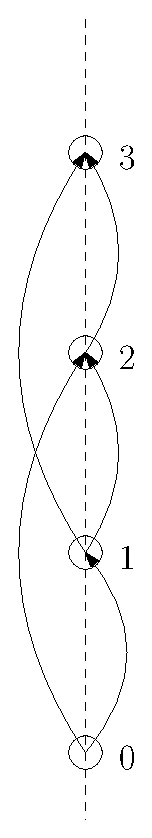
\includegraphics[width=.08\textwidth]{kjumps.eps}\caption{}\label{fig:kjumps}
\end{figure}

When we take $k = 1$, we show that the jumps from $0$ to $2$ can be described by evaluating the jump from $0$ to $1$ and the jump $1$ to $2$ in succession. This also holds for $k = 2$. The jump from $0$ to $3$ can be described by evaluating the jump from $0$ to $2$ and the jump from $2$ to $3$ in succession. This way we proved that we can use \eqref{eq:zkplusfinal} to find an expression for the first-order approximation of the post-impact state for $l$ simultaneous jumps, with $l\in \mathbb{Z}$. Also, we show that multiple constant jump gains will result in a total jump which can also be described by a constant jump gain.

For $l$ simultaneous jumps, we can find the first-order approximation of the post-impact state using

\begin{align}
\ ^{l\leftarrow 0}\zb(\tau) = \ ^{l \leftarrow 0}\Lb(\zb^{0}(\tau),\vb(\tau),\tau) = \ ^{l\leftarrow 0}\Gb\zb^{0}(\tau) + \sum_{i=0}^{l-1}\left(\ ^{l\leftarrow i+1}\Gb\ ^{i+1 \leftarrow i}\boldsymbol{J}\vb^{i}(\tau)\right),\label{eq:ljumps}
\end{align}

where the superscript
\begin{align}
b\leftarrow a =b\leftarrow (b-1) \leftarrow \cdots \leftarrow (a+1) \leftarrow a,
\end{align}

and
\begin{align}
^{b\leftarrow a}\Gb &=\ ^{b\leftarrow (b-1)}\Gb\cdots\ ^{(a+2)\leftarrow (a+1)}\Gb^{(a+1)\leftarrow a}\Gb,\\
^{b\leftarrow a}\Jb &=\ ^{b\leftarrow (b-1)}\Jb\cdots\ ^{(a+2)\leftarrow (a+1)}\Jb^{(a+1)\leftarrow a}\Jb.
\end{align}

\section{Positive homogeneity}\label{app:poshom}
The first order approximation of the perturbed trajectory $\xb_\epsilon$ can be found using $\alphab + \epsilon\zb$, with

\begin{align}
^{s^{k-1}}\dot{\zb} &=\ ^{s^{k-1}}\Ab(t)\ ^{s^{k-1}}\zb +\ ^{s^{k-1}}\Bb(t)\ ^{s^{k-1}}\vb,\nonumber\\
^{s^{k}}\zb &= ^{s^{k}\leftarrow s_{k-1}}\Hb\left(^{s^{k-1}}\zb,t\right),\label{eq:PHdyn}\\
^{s^{k}}\dot{\zb} &=\ ^{s^{k}}\Ab(t)\ ^{s^{k}}\zb +\ ^{s^{k}}\Bb(t)\ ^{s^{k-1}}\vb,\nonumber
\end{align}
where
\begin{align}
^{s^{k}}\Ab(t) &= D_1\ ^{s^{k}}\fb\left(\ ^{s^{k}}\alphab(t),\ ^{s^{k}}\mub(t)\right),\\
^{s^{k}}\Bb(t) &= D_2\ ^{s^{k}}\fb\left(\ ^{s^{k}}\alphab(t),\ ^{s^{k}}\mub(t)\right).
\end{align}

When we look at \eqref{eq:PHdyn}, the continuous dynamics of the system are linear. Because of the conewise constant jump gain however, this linearity property is lost. We can see this by looking at the general solution of \eqref{eq:PHdyn}. A system $f(x,u)$ with state $x$ and input $u$ is linear if $f(x_1,v_1) + f(x_2,v_2) = f(x_1+x_2,v_1+v_2)$. Two solutions of \eqref{eq:PHdyn} before jump are

\begin{align}
^{s^{k-1}}\zb_1(\tau) &= \ ^{s^{k-1}}\phib(t,t_0)\ ^{s^{k-1}}\zb_1(t_0) + \int_{t_0}^\tau \left[\ ^{s^{k-1}}\phib(t,s)\ ^{s^{k-1}}\Bb(s)\vb_1(s)\right]ds,\\
^{s^{k-1}}\zb_2(\tau) &= \ ^{s^{k-1}}\phib(t,t_0)\ ^{s^{k-1}}\zb_2(t_0) + \int_{t_0}^\tau \left[\ ^{s^{k-1}}\phib(t,s)\ ^{s^{k-1}}\Bb(s)\vb_2(s)\right]ds,
\end{align}
with $t_0$ the initial time and $\tau$ the jump time.
When we add these solutions together we find
\begin{multline}
^{s^{k-1}}\zb_1(\tau) + \ ^{s^{k-1}}\zb_2(\tau) = \ ^{s^{k-1}}\phib(t,t_0)\left(\ ^{s^{k-1}}\zb_1(t_0) + \ ^{s^{k-1}}\zb_2(t_0)\right) \\+ \int_{t_0}^\tau \left[\ ^{s^{k-1}}\phib(t,s)\ ^{s^{k-1}}\Bb(s)\left(\vb_1(s) + \vb_2(s)\right)\right]ds,
\end{multline}
which is equal to the solution of $^{s^{k-1}}\zb_3(t_0) = ^{s^{k-1}}\zb_1(t_0) + ^{s^{k-1}}\zb_2(t_0)$ with $\vb_3(t) = \vb_1(t) + \vb_2(t)$. When $^{s^{k-1}}\zb_1$ jumps with $\Gb^1(\zb,\tau)$ and $^{s^{k-1}}\zb_1(\tau)$ jumps with $\Gb^2(\zb,\tau)$ we find the solutions post jump to be
\begin{align}
^{s^{k}}\zb_1(\tau) &= \ ^{s^{k}}\phib(t,t_0)\ \Gb^1(^{s^{k-1}}\zb_1(t_0),\tau) + \int_{t_0}^\tau \left[\ ^{s^{k}}\phib(t,s)\ ^{s^{k}}\Bb(s)\vb_1(s)\right]ds,\label{eq:z1sol}\\
^{s^{k}}\zb_2(\tau) &= \ ^{s^{k}}\phib(t,t_0)\ \Gb^2(^{s^{k-1}}\zb_2(t_0),\tau) + \int_{t_0}^\tau \left[\ ^{s^{k}}\phib(t,s)\ ^{s^{k}}\Bb(s)\vb_2(s)\right]ds,
\end{align}
which when added together results in
\begin{multline}
^{s^{k}}\zb_1(\tau) + \ ^{s^{k}}\zb_2(\tau) = \ ^{s^{k}}\phib(t,t_0)\left(\Gb^1 \ ^{s^{k-1}}\zb_1 + \Jb^1\ ^{s^{k-1}}\vb_1 + \Gb^2 \ ^{s^{k-1}}\zb_2 + \Jb^2\ ^{s^{k-1}}\vb_2\right) \\+ \int_{t_0}^\tau \left[\ ^{s^{k}}\phib(t,s)\ ^{s^{k}}\Bb(s)\left(\vb_1(s) + \vb_2(s)\right)\right]ds.\label{eq:soladd}
\end{multline}
Here we see that the solution of $^{s^{k-1}}\zb_3(t_0) = ^{s^{k-1}}\zb_1(t_0) + ^{s^{k-1}}\zb_2(t_0)$ with $\vb_3(t) = \vb_1(t) + \vb_2(t)$, which jumps with $\Gb_3(\zb,\tau)$, is only the equal to \eqref{eq:soladd} if $\Gb_1(\zb,\tau) = \Gb_2(\zb,\tau) = \Gb_3(\zb,\tau)$. In other words, the system only maintains its linearity after jump if the jump maps are equal for each ante jump state. Because this is generally not true, we show that the system is positive homogeneous for any jump gains. A system $f(x,u)$ with state $x$ and input $u$ is called positive homogeneous, when $\alpha f(x,u) = f(\alpha x, \alpha u)$. If we multiply \eqref{eq:z1sol} with a constant $\alpha$, we find
\begin{align}
^{s^{k}}\zb_1(\tau) &= \alpha \ ^{s^{k}}\phib(t,t_0)\ \left(\Gb^1 \ ^{s^{k-1}}\zb_1 + \Jb^1\ ^{s^{k-1}}\vb_1\right) + \alpha\int_{t_0}^\tau \left[\ ^{s^{k}}\phib(t,s)\ ^{s^{k-1}}\Bb(s)\vb_1(s)\right]ds.\label{eq:alphaz1sol}
\end{align}
If we now look at the solution for $\zb_4(t_0) = \alpha\zb_1(t_0)$ with $\vb_4(t) = \alpha\vb_1(t)$ jumping with $\Gb^4(\tau)$, and using the fact that $\Gb^4(\tau) = \Gb^1(\tau)$ since the gains are conewise constant as illustrated in Figure~\ref{fig:cone}, we find the same solution as \eqref{eq:alphaz1sol}. This shows that \eqref{eq:PHdyn} is positive homogeneous for any conewise constant jump gain $^{s^{k}\leftarrow s^{k-1}}\Hb\left(^{s^{k-1}}\zb,t\right)$. Hence the name, positive homogenization. 

%% New chapter %%
%\pagestyle{fancyreport}
%\cleartooddpage
%\pagestyle{fancyreport}
%\chapter{Verification of Assumptions}\label{app:assumptions}

%% New chapter %%
%\pagestyle{fancyreport}
%\cleartooddpage
%\pagestyle{fancyreport}
%\chapter{Simulation Design}
%\section{System dynamics}

%\section{Reference trajectory design}

%\section{Sensitivity analysis}
\end{document}